%sri
% This is LLNCS.DEM the demonstration file of
% the LaTeX macro package from Springer-Verlag
% for Lecture Notes in Computer Science,
% version 2.4 for LaTeX2e as of 16. April 2010
%
\documentclass{llncs}
%
\usepackage{makeidx}  % allows for indexgeneration
\usepackage{graphicx}
%
\begin{document}

\mainmatter              % start of the contributions
%
\title{As Much Resilience As You Want: \\A Resilient Legion}
%
\titlerunning{Resilience in Legion}
 
\author{Karthik Murthy \and
Mike Bauer \and 
Todd Warszawski\and 
Wonchan Lee \and
Elliott Slaughter \and
Sean Treichler \and
Alex Aiken
}
%
\authorrunning{Karthik Murthy et al.} 
\institute{Stanford University, USA,\\
%\email{kmurthy@stanford.edu}
}

\maketitle              % typeset the title of the contribution

\begin{abstract} 
Resilient is an important aspect of scaling applications on
large clusters. As we approach parallelism profiles of several millions and long running applications, we need to ensure that ineffect ``we reach the end".
Defining the policy interaction with the programming model features necessitates that we revisit the memory concistency model. 
Recoverability, a critical step in
resilience, opens the door to optimizations such as speculation. We also
evaluate this.  \dots
\keywords{resilience}
\end{abstract}

%
\section{Introduction}

\section{Resilience Policy}

%sri

\section{Interaction of Resilience Policy with Legion Features} 

which are the legion features of importance ?

put a figure of interaction.

what is the memory consistency angle here ?

what does it mean to advance the commit wavefront

Resilience is a tangling of the lifetime of a task and a region snapshot- 
1) when can we advance a commit wavefront ?
2) whats the lifetime of a region-instance snapshot ?

on this front, we see it as a two-step process a) define a consistent cut of tasks problem, b) commit any task strictly behind this wavefront c) garbage collect any snapshot that serves as input to any task that is already committed

consistent cut of tasks that can be part of the commit wavefront: 
a set of tasks whose inputs are need\_preserve'ed, or they are strictly post-dominated by tasks whose inputs are need\_preserved.  

3) what about copy/index/tasks ?
copy local to local follows the above semantics
copy local to remote get committed immediately after successful execution.
index launch tasks, actually feel need not be in the task graph, unless virtual mapping is used. they can be garbage collected immediately after all child tasks are included in the dependence analysis wavefront
  - I am thinking we will never have a case where are relaunching the index launch, since hte child tasks either are part of the committed wavefront or are not (pending a discussion on phase barriers)

Question on what to do about must\_epoch tasks with phase\_barrier inside them ?

answer: restartable phase\_barrier with generation commit callback 


%sri


there are three different wavefronts in Legion, we can speculate on any of them. 


From a speculation perspective, are they different ? 
Are we novel, since we have these three different wavefronts ? 
Can we navigate through this, like the blanks 


1) execution wavefront 
what does it mean to speculate here, does the other steps have to be complete before we do this. 


2) mapping wavefront

3) dependence analysis wavefront


-- see mike's 6 wavefront answer.

There are three different wavefronts, there could

 
mike - speculation is more about tracking the resolution wavefront while resilience is more about tracking the commit wavefront, but the when things go bad, then i think the machinery to restart the mapping and execution wavefronts should be the same


\section{Implementation}

%sri

\section{Experiments}

\subsection{Index Tasks}

\paragraph{Growth of memory as execution proceeds}
\paragraph{Performance overhead as execution proceeds}



\begin{center}
 \begin{tabular}{||c | c | c | c||} 
 \hline
 NumIter& No Resl No lg:res & No Res With lg:res & Res No lg:res \\ [0.25ex] 
 \hline\hline
100 &  7.2 & 6.6 & 23.6\\ 
 \hline
200 &  13.8 & 13.3 & 46.3\\ 
 \hline
400 &  26.1 & 26.5 & 94.4\\ 
 \hline
800 &  55 & 53 & 186.8\\ 
 \hline
1000 &  65 & 66 & 239.9\\ [1ex] 
 \hline
\end{tabular}
\end{center}

\begin{figure}
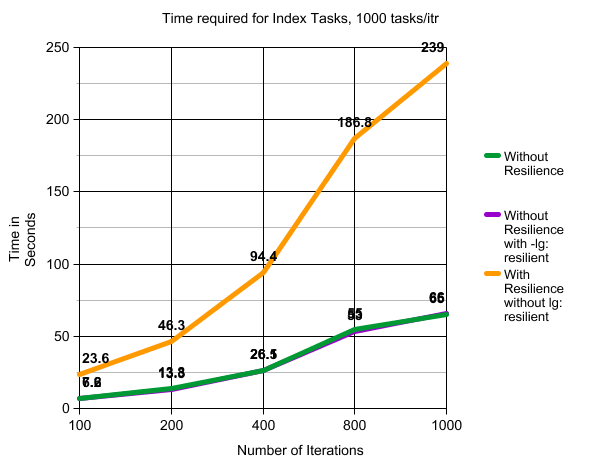
\includegraphics[width=\textwidth]{images/index_tasks_time.png}
\caption{Total time taken by 02\_index\_tasks. Time in Seconds, 1000 tasks/index launch }
\end{figure}


\begin{center}
 \begin{tabular}{||c | c | c | c||} 
 \hline
 NumIter& No Resl No lg:res & No Res With lg:res & Res No lg:res \\ [0.25ex] 
 \hline\hline
100 &  18 & 140 & 107 \\ 
 \hline
200 &  22 & 263 & 176 \\ 
 \hline
400 &  24 & 509 & 245 \\ 
 \hline
800 &  26 & 1002 & 428\\ 
 \hline
1000 & 26 & 1248 & 518\\ [1ex] 
 \hline
\end{tabular}
\end{center}

\begin{figure}
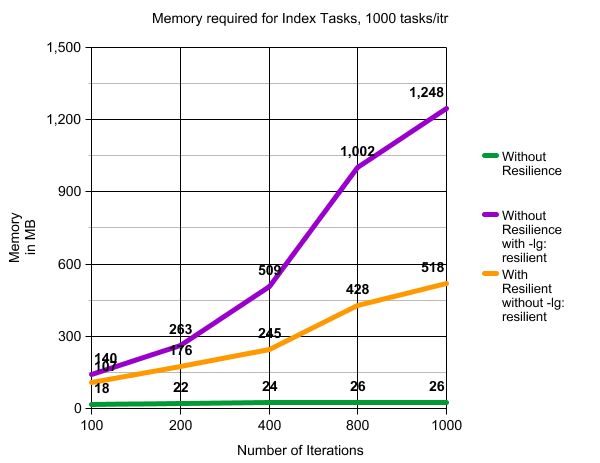
\includegraphics[width=\textwidth]{images/index_tasks_memory.png}
\caption{Total Memory footprint by 02\_index\_tasks. Memory in MB, 1000 tasks/index launch.}
\end{figure}





\subsection{Stencil}



\subsection{local recover vs global recovery}

\subsection{compute/comm vs no-failure/single failure/multi-failure}

\subsection{S3D, Pennant, Stencil, Circuit}

\subsection{Some Interesting Task Graphs for Recovery}




\subsection{Experiments}

pennant, stencil, miniAero (better understood) /Circuit, 
- limit the failure to the before

\section{Adaptive Resilience}

\subsection{Resilience Policy Implemented via Mapper: Example 1 Generic}

\subsection{Resilience Policy Implemented via Mapper: Example 2 UT Austin}
\subsubsection{Interaction of need\_preserve with the commit wavefront}
\subsubsection{Obtaining dependence graph in the mapper before calling need\_preserve} 

\section{Related Work}

\section{Conclusion}

%
% ---- Bibliography ----
%

\begin{thebibliography}{5}
%
\bibitem {clar:eke}
Clarke, F., Ekeland, I.:
Nonlinear oscillations and
boundary-value problems for Hamiltonian systems.
Arch. Rat. Mech. Anal. 78, 315--333 (1982)

\bibitem {rab}
Rabinowitz, P.:
On subharmonic solutions of a Hamiltonian system.
Comm. Pure Appl. Math. 33, 609--633 (1980)

\end{thebibliography}

\clearpage
%\addtocmark[2]{Author Index} % additional numbered TOC entry
%\renewcommand{\indexname}{Author Index}
%\printindex
%\clearpage
%\addtocmark[2]{Subject Index} % additional numbered TOC entry
%\markboth{Subject Index}{Subject Index}
%\renewcommand{\indexname}{Subject Index}
%\input{subjidx.ind}
\end{document}
